\documentclass[preprint,12pt]{elsarticle}

\usepackage{amsmath}
\usepackage{booktabs}
\usepackage{float}
\usepackage{graphicx}
\usepackage{hyperref}

\journal{Journal target to be confirmed before submission}
\biboptions{numbers,sort&compress}

\begin{document}

\begin{frontmatter}

\title{Uncertainty-Aware Bearing-Only Passive Localization with Credibility-Guided Measurement Selection for Collaborative UAV Sensing}

\author[inst1]{Zengye Su\corref{cor1}}
\ead{Corresponding e-mail to be confirmed before submission}
\author[inst1]{Yudan Nie}
\author[inst2]{Zilu Zhou}
\cortext[cor1]{Corresponding author.}
\address[inst1]{Affiliation to be confirmed before submission}
\address[inst2]{Guangzhou College of Commerce, Guangzhou 511363, China}

\begin{abstract}
Passive bearing-only localization remains attractive for collaborative unmanned aerial vehicle (UAV) sensing in GNSS-denied or electromagnetically silent missions, but its practical usefulness is limited by uncertain measurements. In realistic deployments, some bearings can be biased, missing, or grossly corrupted, so fusing every available observation may destabilize the estimate instead of improving it. This paper presents an uncertainty-aware algorithmic framework for passive bearing localization that couples a geometry-preserving robust estimator with a credibility-guided measurement-selection layer. The robust core combines multi-candidate geometric initialization, trimming-aware residual suppression, iterative reweighting, and optional common-bias correction. A subsequent selection stage ranks measurement subsets using observability quality, angular diversity, geometry isotropy, and residual-derived reliability, then re-estimates the target from the chosen subset. Synthetic experiments under biased, outlier, mixed-corruption, multi-formation, and sensor-scaling settings show that the robust core markedly improves over least squares in the regimes that matter most for passive sensing. In the fixed-budget selection benchmark, the proposed policy reduces the overall median error to 0.4977, compared with 0.7491 for random subsets, 0.5676 for angular-spread greedy selection, and 0.5200 for FIM/CRLB-greedy selection, while achieving the best success rate at the 1.0-error threshold among the tested subset policies. The comparison with all-sensor estimation is mixed, indicating that measurement selection is most useful when part of the bearing set is unreliable rather than universally preferable. The resulting study is best understood as a reproducible passive-localization framework for uncertain observations and a practical bridge toward stronger active sensing.
\end{abstract}

\begin{keyword}
Passive localization \sep bearing-only localization \sep UAV swarm \sep collaborative sensing \sep robust estimation \sep uncertainty-aware sensing \sep measurement selection \sep GNSS-denied navigation
\end{keyword}

\end{frontmatter}

\section{Introduction}

Collaborative unmanned aerial vehicle (UAV) systems are increasingly expected to operate in GNSS-denied, low-emission, or electromagnetically silent environments. In such settings, passive bearing-only or angle-of-arrival sensing remains attractive because it supports target search, emergency observation, and low-detectability surveillance without requiring active emission \cite{kramaric2025comprehensive,liu2025survey,avola2024uav}. The practical difficulty is not simply geometric triangulation itself, but the fact that real bearings are unreliable: some observations can be biased, intermittently missing, or contaminated by large errors, and a small number of bad bearings can trigger large localization failures \cite{wang2025bio,chen2025error,li2025bearing}.

Recent literature shows two strong development trends. One line pushes toward system-level cooperative localization through formation constraints, distributed estimation, and factor-graph inference \cite{li2026formation,yang2024distributed}. Another line improves sensing geometry through observability-aware trajectory design, CRLB-driven path optimization, sensor-bias calibration, or passive node selection \cite{peng2024trajectory,he2019trajectory,chen2025variable,wang2025bio,xing2025node}. These directions are important, but they do not remove a lighter-weight practical need: in a single passive localization cycle, how should a UAV team localize robustly when the available bearings are uncertain and not all of them deserve equal trust?

This paper targets that problem. It presents an uncertainty-aware bearing-only passive localization framework that keeps geometric reasoning explicit while improving robustness under degraded measurements. The method first stabilizes estimation through multi-candidate initialization, trimming-aware residual handling, and iterative reweighting, then performs credibility-guided measurement selection based on observability quality and residual reliability. The paper does not claim to replace graph-based cooperative inference or long-horizon trajectory planning. Instead, it shows that a lightweight algorithmic framework can materially improve passive localization under uncertain observations and can produce a reusable baseline for stronger active-sensing extensions.

The main contributions are fourfold:
\begin{itemize}
\item an interpretable robust bearing-only passive localization framework for collaborative UAV sensing under biased, missing, and outlier-corrupted measurements;
\item a credibility-guided measurement-selection strategy that explicitly treats some bearings as more informative and trustworthy than others, instead of assuming that every available observation should always be fused;
\item a degraded-regime benchmark protocol covering regime comparison, ablation, formation generalization, sensitivity sweeps, sensor-count scaling, paired significance testing, and observability-oriented interpretation;
\item a restrained literature-grounded positioning of the method as a simulation-validated algorithmic framework for uncertain passive sensing rather than a universal replacement for heavier system-level localization pipelines.
\end{itemize}

The remainder of this paper is organized as follows. Section~2 reviews recent work on passive localization, observability-oriented planning, and cooperative UAV localization. Section~3 formulates the uncertain-measurement localization problem. Section~4 introduces the robust estimator and credibility-guided measurement-selection strategy. Sections~5 and 6 report the experimental design and results, and Sections~7 and 8 discuss the scope and conclude the paper.

\section{Related Work}

Recent surveys confirm that UAV localization remains an active topic under GNSS degradation, heterogeneous sensing, and cooperative mission constraints \cite{kramaric2025comprehensive,liu2025survey,avola2024uav}. Within this broader area, passive localization remains especially relevant in low-emission or electromagnetically silent scenarios, including recent UAV formation studies on azimuth-only positioning and system-level node selection for passive target localization \cite{li2025bearing,xing2025node}. Recent UAV formation papers therefore still study azimuth-only passive positioning, showing that the application background is contemporary rather than outdated \cite{li2025bearing}.

Another active thread in the literature seeks better geometry or better decisions. Observability-aware path design, sensor-bias calibration, active trajectory optimization, and CRLB-driven path optimization have been studied to improve bearing-only localization quality or broader passive-target-localization performance \cite{peng2024trajectory,wang2025bio,he2019trajectory,chen2025variable,xing2025node}. These papers show that informative geometry matters, but they typically emphasize motion planning, path design, or system-level sensing allocation rather than the reliability triage of a fixed bearing set.

At the same time, cooperative localization research is becoming more system-oriented. Representative examples include formation-constrained localization, distributed estimation, and factor-graph inference for UAV teams \cite{li2026formation,yang2024distributed}. Those directions are stronger at the system level, but they also impose a heavier modeling and integration burden than a lightweight passive estimator. Compared with them, the present work focuses on a narrower question: how far a geometry-preserving robust estimator can go when it explicitly accounts for corrupted bearings and is equipped with a lightweight measurement-selection layer. This positioning is intentional. The paper does not replace graph optimization or long-horizon active planning; it provides a robust passive-localization core and a reproducible benchmark that clarify when such a lighter framework is already useful.

\section{Problem Formulation}

We consider a single passive localization cycle for a collaborative UAV team. Let $N$ observing UAVs be located at positions
\begin{equation}
s_i = [x_i, y_i]^T, \quad i = 1, \dots, N,
\end{equation}
and a target position
\begin{equation}
p = [x, y]^T.
\end{equation}
Each valid observer provides a bearing-only measurement
\begin{equation}
\theta_i = \operatorname{atan2}(y-y_i, x-x_i) + b + \epsilon_i + o_i,
\end{equation}
where $b$ is a common angular bias term, $\epsilon_i$ denotes nominal noise, and $o_i$ models occasional gross corruption. Some measurements may be unavailable because of missed detections, occlusion, or communication loss.

For a candidate target position $p$, the predicted bearing from observer $i$ is
\begin{equation}
\hat{\theta}_i(p)=\operatorname{atan2}(y-y_i, x-x_i),
\end{equation}
and the wrapped residual under common bias $b$ is
\begin{equation}
r_i(p,b)=\operatorname{wrap}\!\left(\hat{\theta}_i(p)-\theta_i-b\right),
\end{equation}
where $\operatorname{wrap}(\cdot)$ maps an angle to $(-\pi,\pi]$.

The objective is to recover $p$ under uncertain measurements while controlling failure risk. Two features are important in this paper. First, the estimator should remain stable when some bearings are unreliable. Second, when only a subset of measurements should be retained, the selection rule should prefer bearings that are both informative and credible. The manuscript studies five representative regimes: clean, biased, missing, outlier, and mixed. This setup is aligned with recent passive UAV literature and with observability-oriented bearing-only studies \cite{li2025bearing,wang2025bio,peng2024trajectory}.

\section{Proposed Method}

\subsection{Consensus Geometric Initialization}

Instead of relying on a single closed-form estimate, the method generates several geometric candidates from pairwise bearing intersections and simple aggregation rules. For observer $i$, the bearing ray is
\begin{equation}
\ell_i(\tau_i)=s_i+\tau_i
\begin{bmatrix}
\cos \theta_i\\
\sin \theta_i
\end{bmatrix},
\end{equation}
and pairwise candidates are obtained from the intersections of non-parallel rays. Let $\mathcal{Z}$ denote the valid pairwise intersections. The initializer forms a small candidate pool containing the centroid of $\mathcal{Z}$, the coordinate-wise median of $\mathcal{Z}$, and a trimmed centroid after removing the farthest intersections from the current center. This preserves interpretability while reducing dependence on any one fragile initialization.

\subsection{Trimming-Aware Robust Refinement}

For each candidate, wrapped angular residuals are computed between predicted and observed bearings. The refinement stage minimizes a weighted Huber objective
\begin{equation}
J(p,b;w)=\frac{\sum_{i=1}^{N} w_i \, \rho_{\delta}\!\left(r_i(p,b)\right)}{\sum_{i=1}^{N} w_i},
\end{equation}
with
\begin{equation}
\rho_{\delta}(r)=
\begin{cases}
\frac{1}{2}r^2, & |r|\le \delta,\\
\delta\left(|r|-\frac{1}{2}\delta\right), & |r|>\delta.
\end{cases}
\end{equation}
At each outer iteration, the largest residuals are trimmed according to a trim ratio $\alpha$, and the remaining observations receive reliability weights
\begin{equation}
w_i \leftarrow \max \left(w_{\min}, \min\left(1,\frac{\delta}{|r_i(p,b)|+\varepsilon}\right)\right),
\end{equation}
with trimmed observations forced to zero weight. The target position is then updated by gradient descent on $J(p,b;w)$ using a finite-difference gradient in the current implementation. In practical terms, this stage acts as the uncertainty-handling core of the framework: it attempts to keep the estimate stable even when part of the bearing set is misleading.

\subsection{Optional Common-Bias Correction}

The framework also includes a lightweight circular residual-mean correction term for shared angular bias:
\begin{equation}
b \leftarrow \angle \left(\sum_{i=1}^{N} w_i \exp\!\left(j \tilde{r}_i\right)\right),
\end{equation}
where $\tilde{r}_i=\operatorname{wrap}(\hat{\theta}_i(p)-\theta_i)$. Ablation results show that trimming and robust weighting contribute more strongly than bias correction alone, but the bias term remains useful when corruption is moderate rather than extreme.

\subsection{Credibility-Guided Measurement Selection}

The second stage adds a one-shot measurement-selection layer after the pilot robust estimate. Starting from all currently valid bearings, the method first computes a pilot estimate and its residual pattern. It then scores candidate subsets using four ingredients: weighted observability quality, geometry isotropy, angular diversity, and residual-derived reliability. The chosen subset is finally passed back into the same robust refinement module.

For a subset $\mathcal{S}$, the weighted Fisher-style geometry matrix is
\begin{equation}
\mathbf{F}_{\mathcal{S}}=\sum_{i\in\mathcal{S}} w_i \mathbf{J}_i^T \mathbf{J}_i,
\end{equation}
where $\mathbf{J}_i$ is the bearing Jacobian with respect to the target position. From $\mathbf{F}_{\mathcal{S}}$, the method extracts determinant-based observability, trace, and isotropy
\begin{equation}
\eta_{\mathcal{S}}=\frac{\lambda_{\min}(\mathbf{F}_{\mathcal{S}})}{\lambda_{\max}(\mathbf{F}_{\mathcal{S}})}.
\end{equation}
Angular diversity is measured from the predicted bearing spread within the subset:
\begin{equation}
\nu_{\mathcal{S}}=\frac{2}{|\mathcal{S}|(|\mathcal{S}|-1)\pi}\sum_{i<j,\, i,j\in\mathcal{S}}
\left|\operatorname{wrap}\!\left(\hat{\theta}_i-\hat{\theta}_j\right)\right|.
\end{equation}
Let $\bar{w}_{\mathcal{S}}$ and $\bar{r}_{\mathcal{S}}$ denote the mean reliability and mean absolute residual on the subset. The proposed policy scores candidate subsets using
\begin{equation}
\begin{aligned}
\operatorname{Score}_{\text{prop}}(\mathcal{S}) ={}& 0.95 \log\!\left(1+10^{4}\det(\mathbf{F}_{\mathcal{S}})\right)
+ 0.40 \eta_{\mathcal{S}}
+ 0.25 \nu_{\mathcal{S}} \\
&+ 0.75 \bar{w}_{\mathcal{S}}
+ 0.08 \log\!\left(1+50 \operatorname{tr}(\mathbf{F}_{\mathcal{S}})\right)
- 0.80 \min\!\left(\frac{\bar{r}_{\mathcal{S}}}{0.2}, 2\right).
\end{aligned}
\end{equation}
The \texttt{spread} and \texttt{crlb} baselines reuse subsets of these terms, while the \texttt{random} baseline samples uniformly at the same budget. The implementation starts from the best two-sensor seed subset and then greedily adds sensors until the fixed budget is reached.

This stage should be interpreted as measurement triage rather than universal sensor pruning. Its role is to help in conditions where some available bearings are less trustworthy than others, or where a fixed sensing budget prevents using every observation. The method therefore prefers subsets that are both geometrically informative and less likely to be corrupted by the current residual pattern.

\subsection{Algorithm Summary}

The complete pipeline can be summarized as follows:
\begin{enumerate}
\item generate several geometry-based initial candidates from pairwise line intersections;
\item run trimmed iterative reweighting with optional common-bias correction for each candidate;
\item retain the candidate with the smallest active residual as the pilot robust estimate;
\item compute per-measurement residual reliability from the pilot estimate;
\item greedily select a fixed-budget subset using either the proposed score or a baseline score;
\item rerun robust refinement on the retained subset to produce the final estimate.
\end{enumerate}

\section{Experimental Setup}

All experiments are synthetic and fully reproducible. The benchmark includes common bias, missing observations, outlier corruption, mixed degradation, multiple formation layouts, and scaling in sensor count. Baselines include least squares, robust Huber refinement, particle swarm optimization (PSO), simulated annealing (SA), and the proposed robust bias-trimmed estimator. The fixed-budget selection benchmark additionally compares the proposed measurement-selection policy against random subset selection, angular-spread greedy selection, and FIM/CRLB-guided greedy selection.

The current validation remains simulation-based, and the manuscript is intentionally scoped as an algorithmic paper rather than a platform-level deployment study. The synthetic design is used to isolate uncertainty patterns that are difficult to control separately in real flight tests, while the discussion section explicitly reserves hardware-in-the-loop, replay-based, or field validation as next-stage work.

The evaluation is organized around five scientific questions:
\begin{itemize}
\item Does the method improve robustness under corrupted bearings?
\item Which components actually matter?
\item Does the advantage persist across formation layouts and sensor counts?
\item Are the differences statistically stable?
\item How does geometry quality help explain performance variation?
\end{itemize}

\section{Results}

The strongest gains appear in outlier-rich and mixed regimes. In the outlier setting, the proposed method reduces median error from $1.6290$ to $0.3863$ and eliminates catastrophic failures above $5.0$ in the reported 20-seed summary. In the mixed regime, the median error drops from $1.4863$ to $0.6779$, while paired sign testing against least squares yields $17$ wins and $3$ losses with $p=0.0026$. Against PSO, the comparison is more balanced, which is exactly the honest interpretation this manuscript adopts: the method is a robust and reproducible alternative to fragile classical estimators rather than a universal winner against every heuristic baseline.

The severity sweeps further refine the claim. At outlier rate $0.40$, least squares reaches a median error of $1.9923$, while the proposed method remains at $0.9189$. At nominal noise $\sigma=0.08$, the proposed method remains slightly better than PSO and clearly better than least squares. In contrast, under pure high-bias stress, PSO can still be stronger, indicating that the main advantage of the proposed framework lies in robust corruption handling rather than bias-only compensation.

Formation-generalization and scaling experiments show that the method is not tied to a single idealized geometry. Under random formation, the mixed-regime median error decreases from $2.1047$ to $0.5768$. In scaling experiments, richer collaborative geometry makes the robust core increasingly competitive: for a 12-UAV circular formation, the proposed method achieves $0.4048$ median error versus $2.3359$ for least squares and $0.3348$ for PSO. Under random formations, the robust method outperforms PSO for the 8-, 10-, and 12-UAV settings.

To reduce the risk that the 20-seed summaries are merely small-sample artifacts, a higher-sample follow-up validation was also run for the two most important degraded regimes using 100 seeds. The same qualitative pattern remains. In the outlier regime, Robust-BT versus least squares yields $83$ wins and $17$ losses with sign-test $p=1.31\times10^{-11}$, and the median improvement is $1.6921$ with a bootstrap 95\% interval of approximately $[1.1023,\,2.1663]$. In the mixed regime, Robust-BT versus least squares yields $75$ wins and $25$ losses with $p=5.64\times10^{-7}$ and a median improvement of $0.5511$ with a bootstrap 95\% interval of approximately $[0.1310,\,1.2295]$. Against PSO, the outlier advantage becomes only marginal and the mixed-regime comparison remains unfavorable, which again supports the restrained claim of this paper: the framework is strongly preferable to fragile classical estimation, while its relationship to heuristic global search is competitive and regime-dependent rather than universally dominant.

The measurement-selection experiment is the key extension result, but it should be interpreted carefully. Aggregated over mixed and severe regimes, three formation families, and 8/10/12-UAV settings, the proposed policy achieves an overall median error of $0.4977$, compared with $0.7491$ for random subset selection, $0.5676$ for angular-spread greedy selection, and $0.5200$ for FIM/CRLB-greedy selection. It also attains the best success rate at the 1.0-error threshold among the tested subset policies ($0.8531$ versus $0.8298$ for FIM/CRLB and $0.6200$ for random selection). In the severe-regime slice, the proposed policy improves the mean error from $1.2450$ to $0.9858$ relative to FIM/CRLB selection while reducing the catastrophic-failure rate from $0.0282$ to $0.0188$.

At the same time, the comparison with all-sensor robust estimation is mixed: the proposed policy yields a lower aggregate median error ($0.4977$ versus $0.5510$), but the paired count is $200$ wins versus $222$ losses. This is an important boundary rather than a weakness to hide. It indicates that measurement selection is not a universal replacement for using every available bearing. Instead, it is most useful when measurement credibility varies or when the sensing process is budgeted and a smaller, cleaner subset is preferable to indiscriminate fusion.

An additional observability-oriented analysis was performed for interpretation only. Circular formations have higher median isotropy than random ones, and stronger estimators benefit more consistently from informative geometry than least squares. This observability section is intentionally modest: it does not claim a theorem, but it does clarify why richer sensing geometry makes the robust estimator's advantages easier to realize. Runtime results are retained only as an implementation-cost reference and are not part of the main scientific claim.

\begin{figure}[t]
\centering
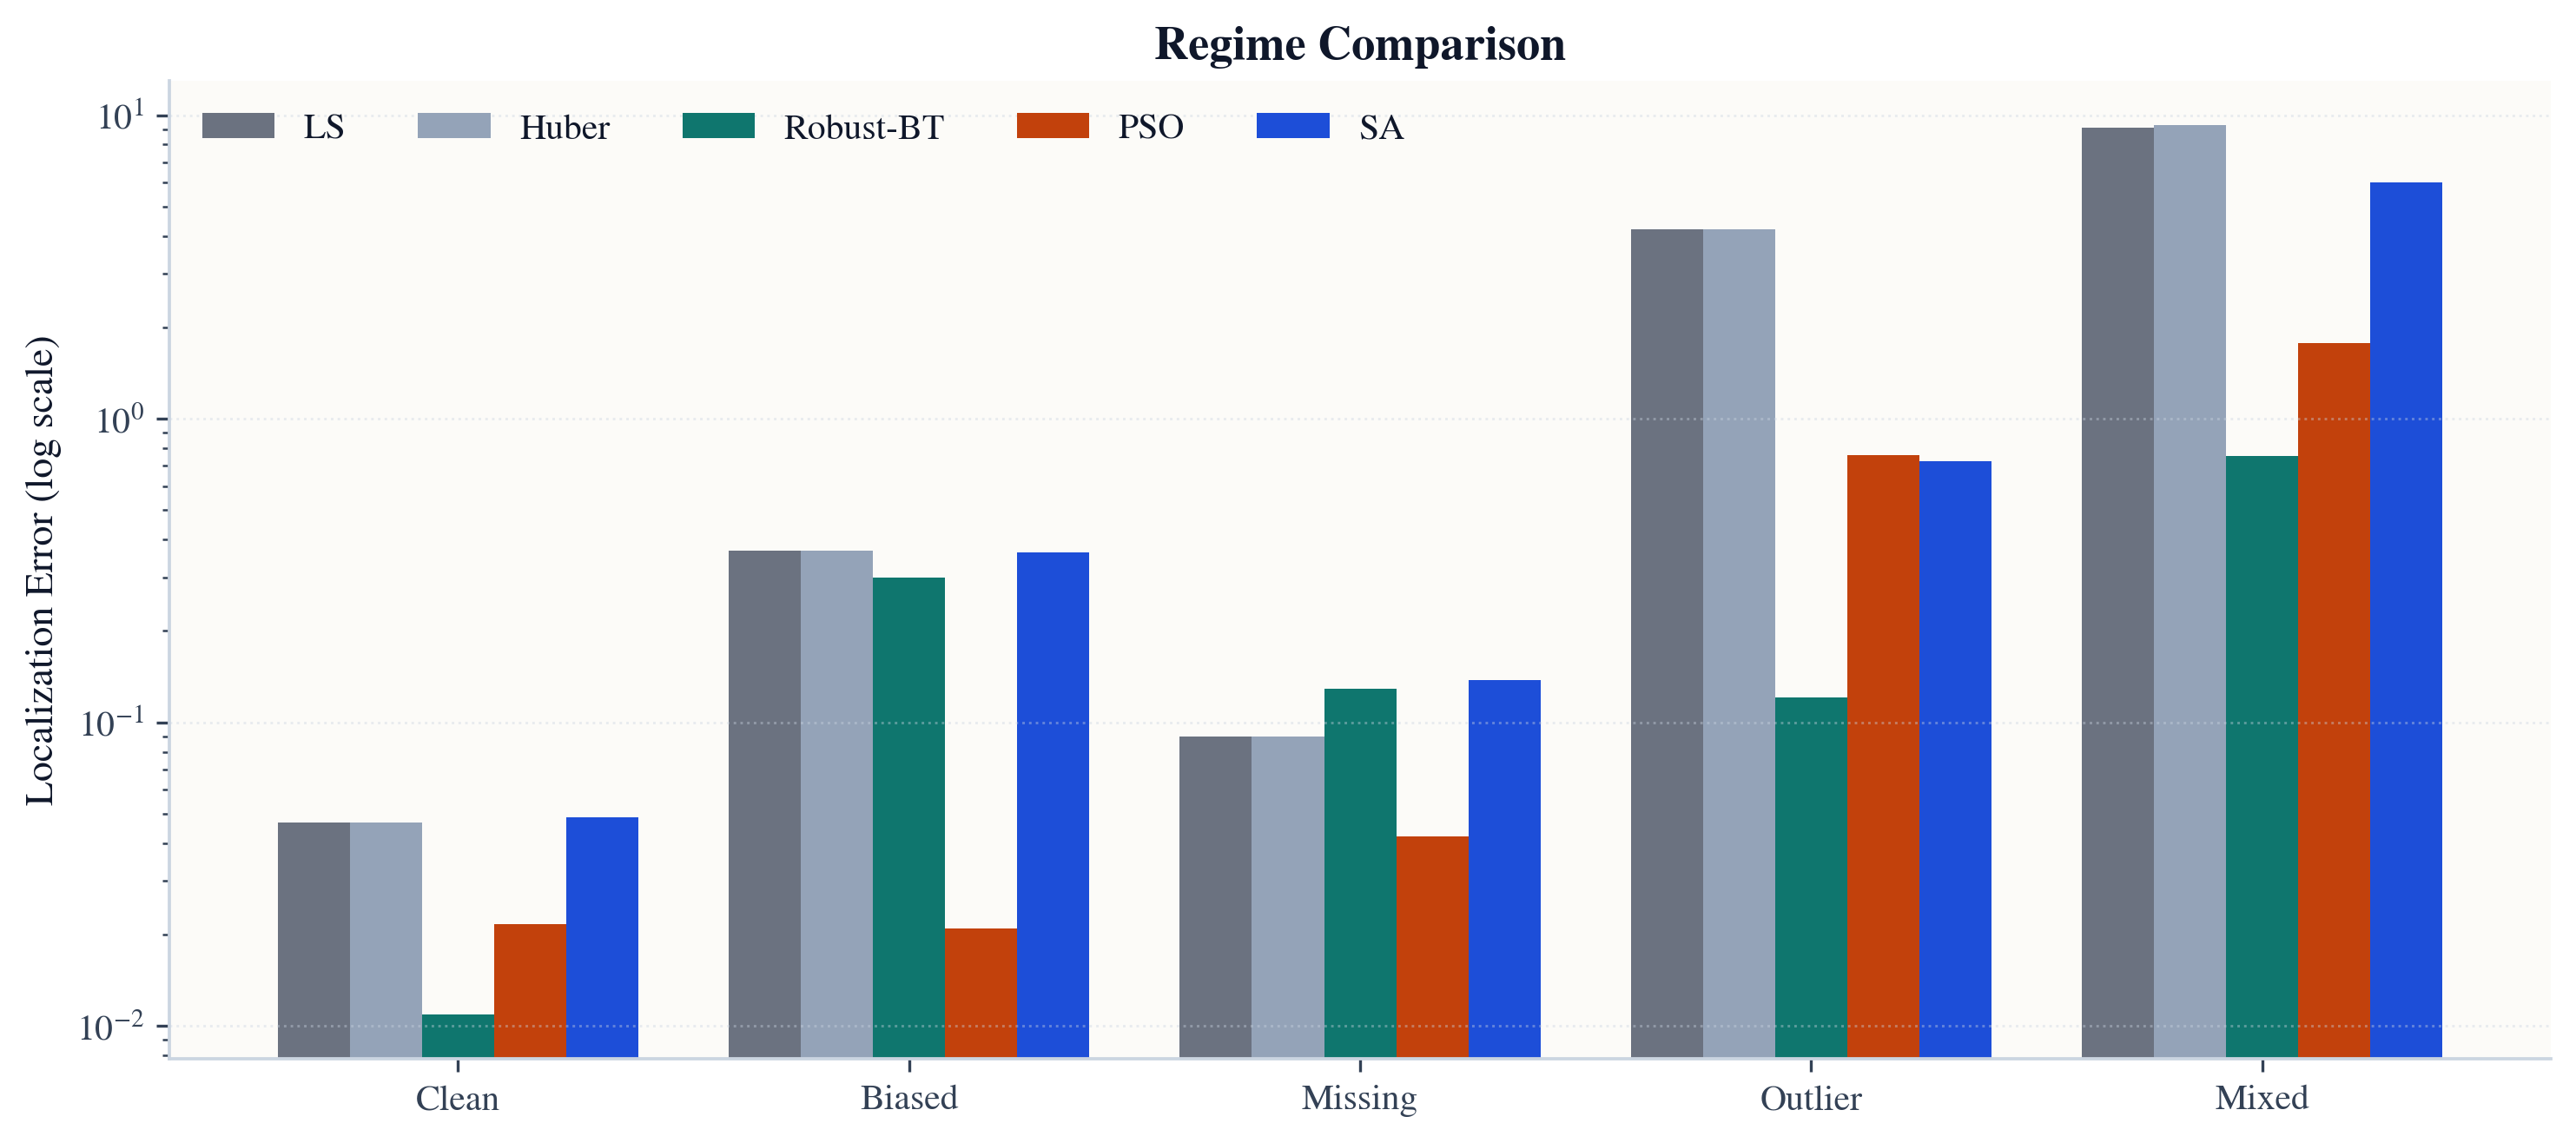
\includegraphics[width=0.95\linewidth]{../figures/figure_regime_comparison.png}
\caption{Regime comparison under clean, biased, missing, outlier, and mixed measurements.}
\label{fig:regime}
\end{figure}

\begin{figure}[t]
\centering
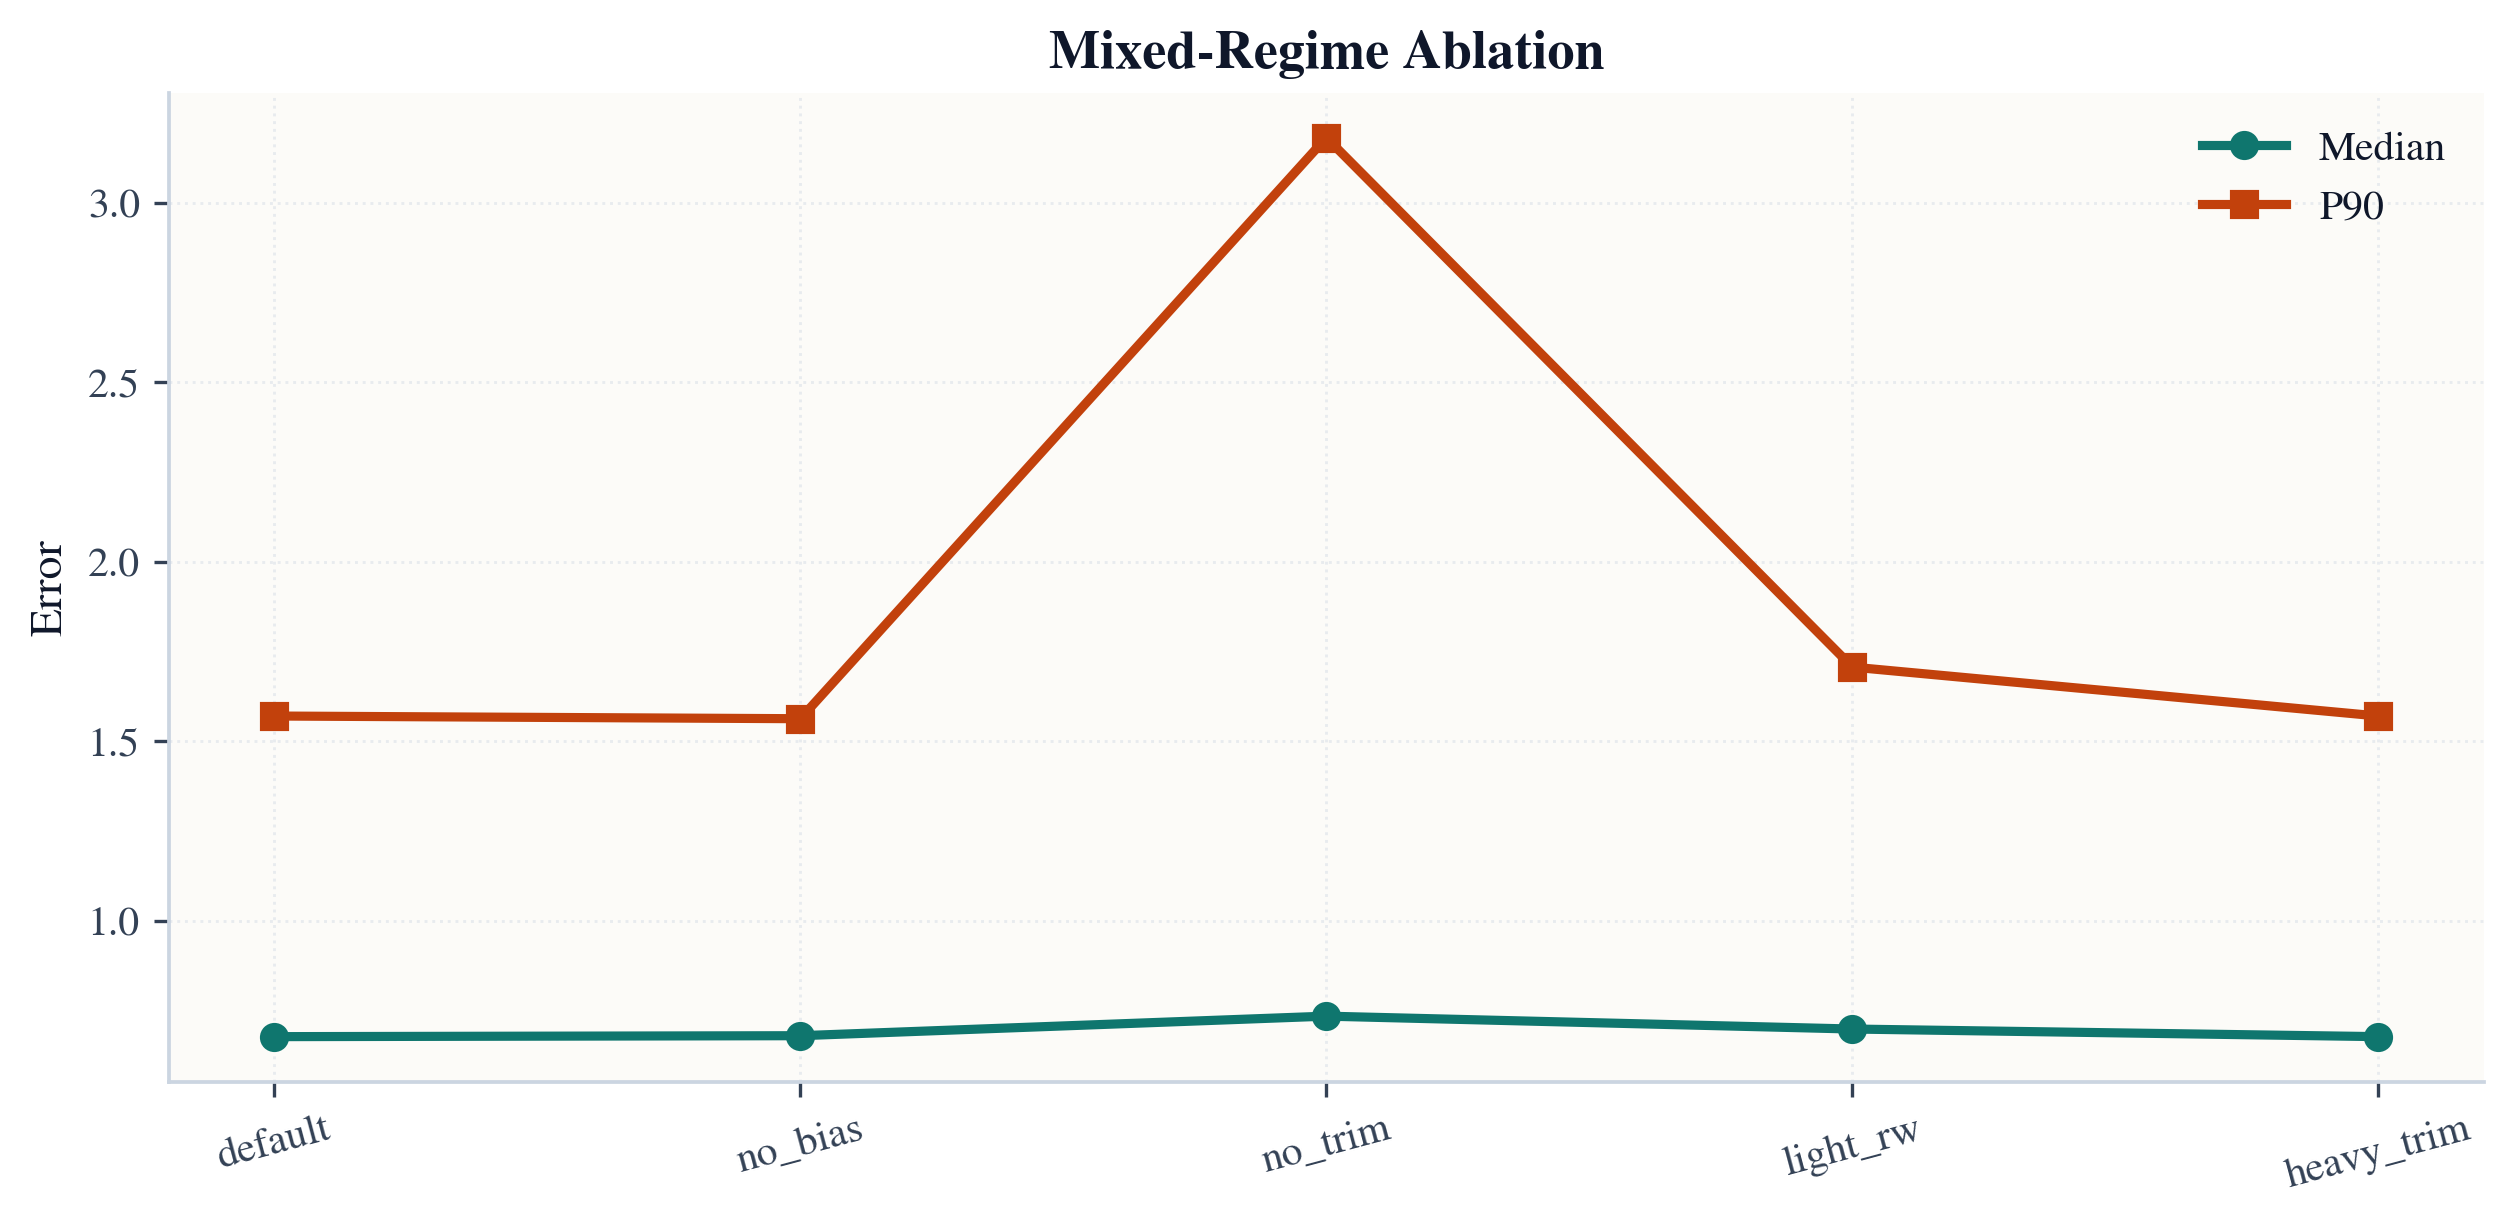
\includegraphics[width=0.8\linewidth]{../figures/figure_ablation_mixed.png}
\caption{Mixed-regime ablation of the proposed robust framework.}
\label{fig:ablation}
\end{figure}

\begin{figure}[t]
\centering
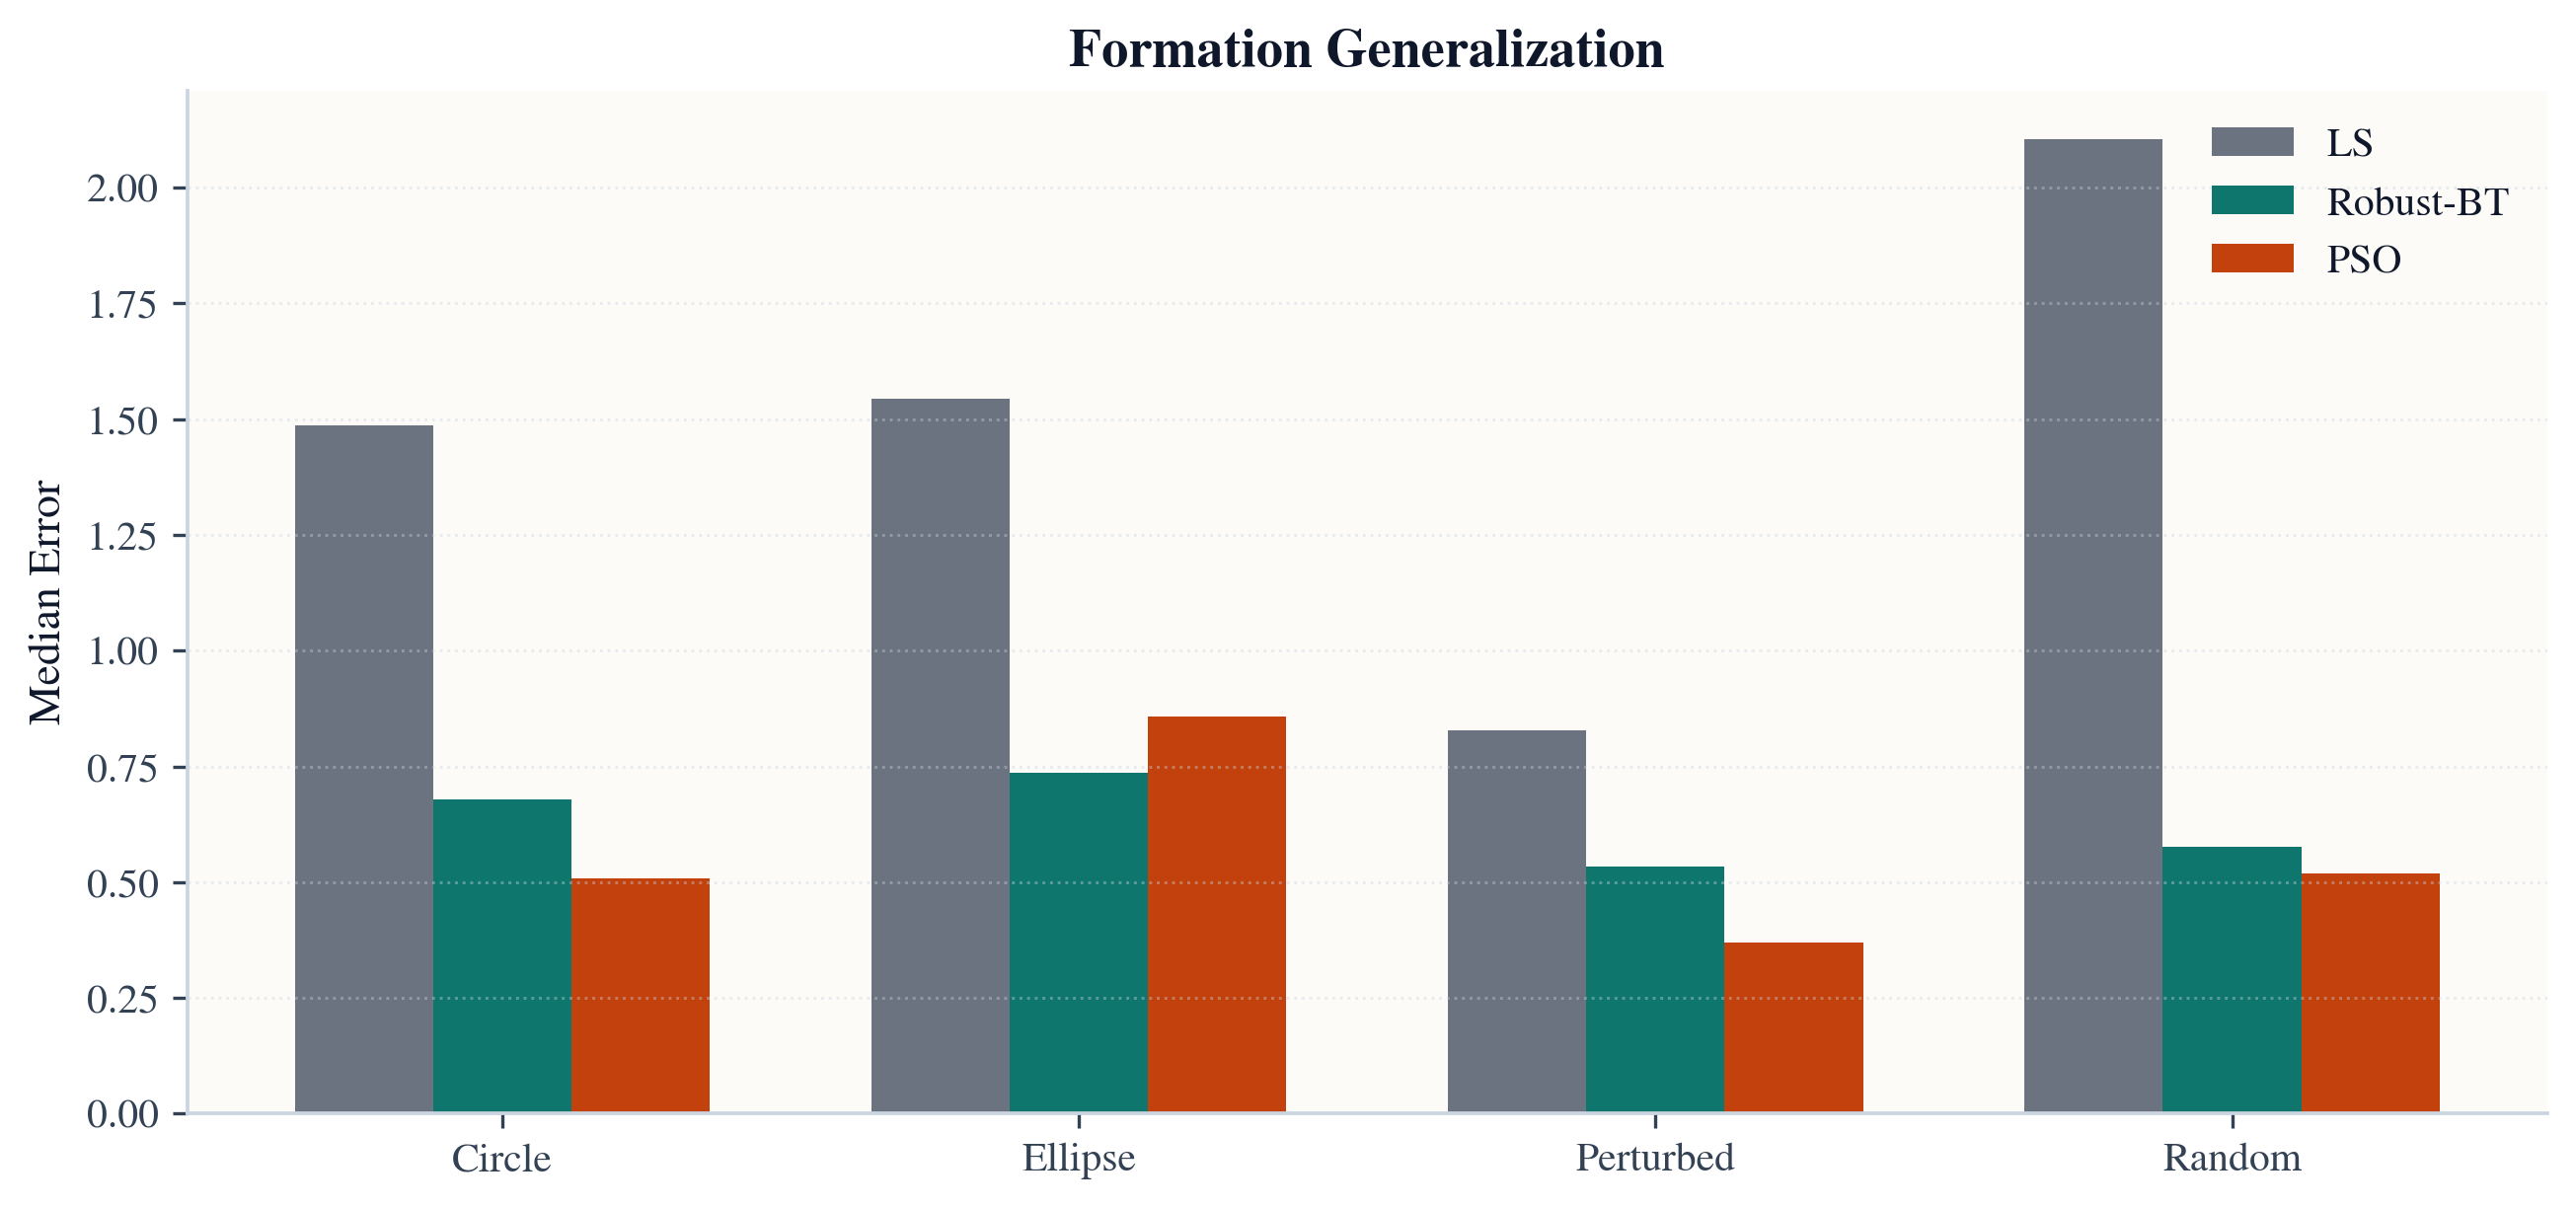
\includegraphics[width=0.82\linewidth]{../figures/figure_formation_generalization.png}
\caption{Formation generalization across circular, elliptical, perturbed, and random swarm layouts.}
\label{fig:formation}
\end{figure}

\begin{figure}[t]
\centering
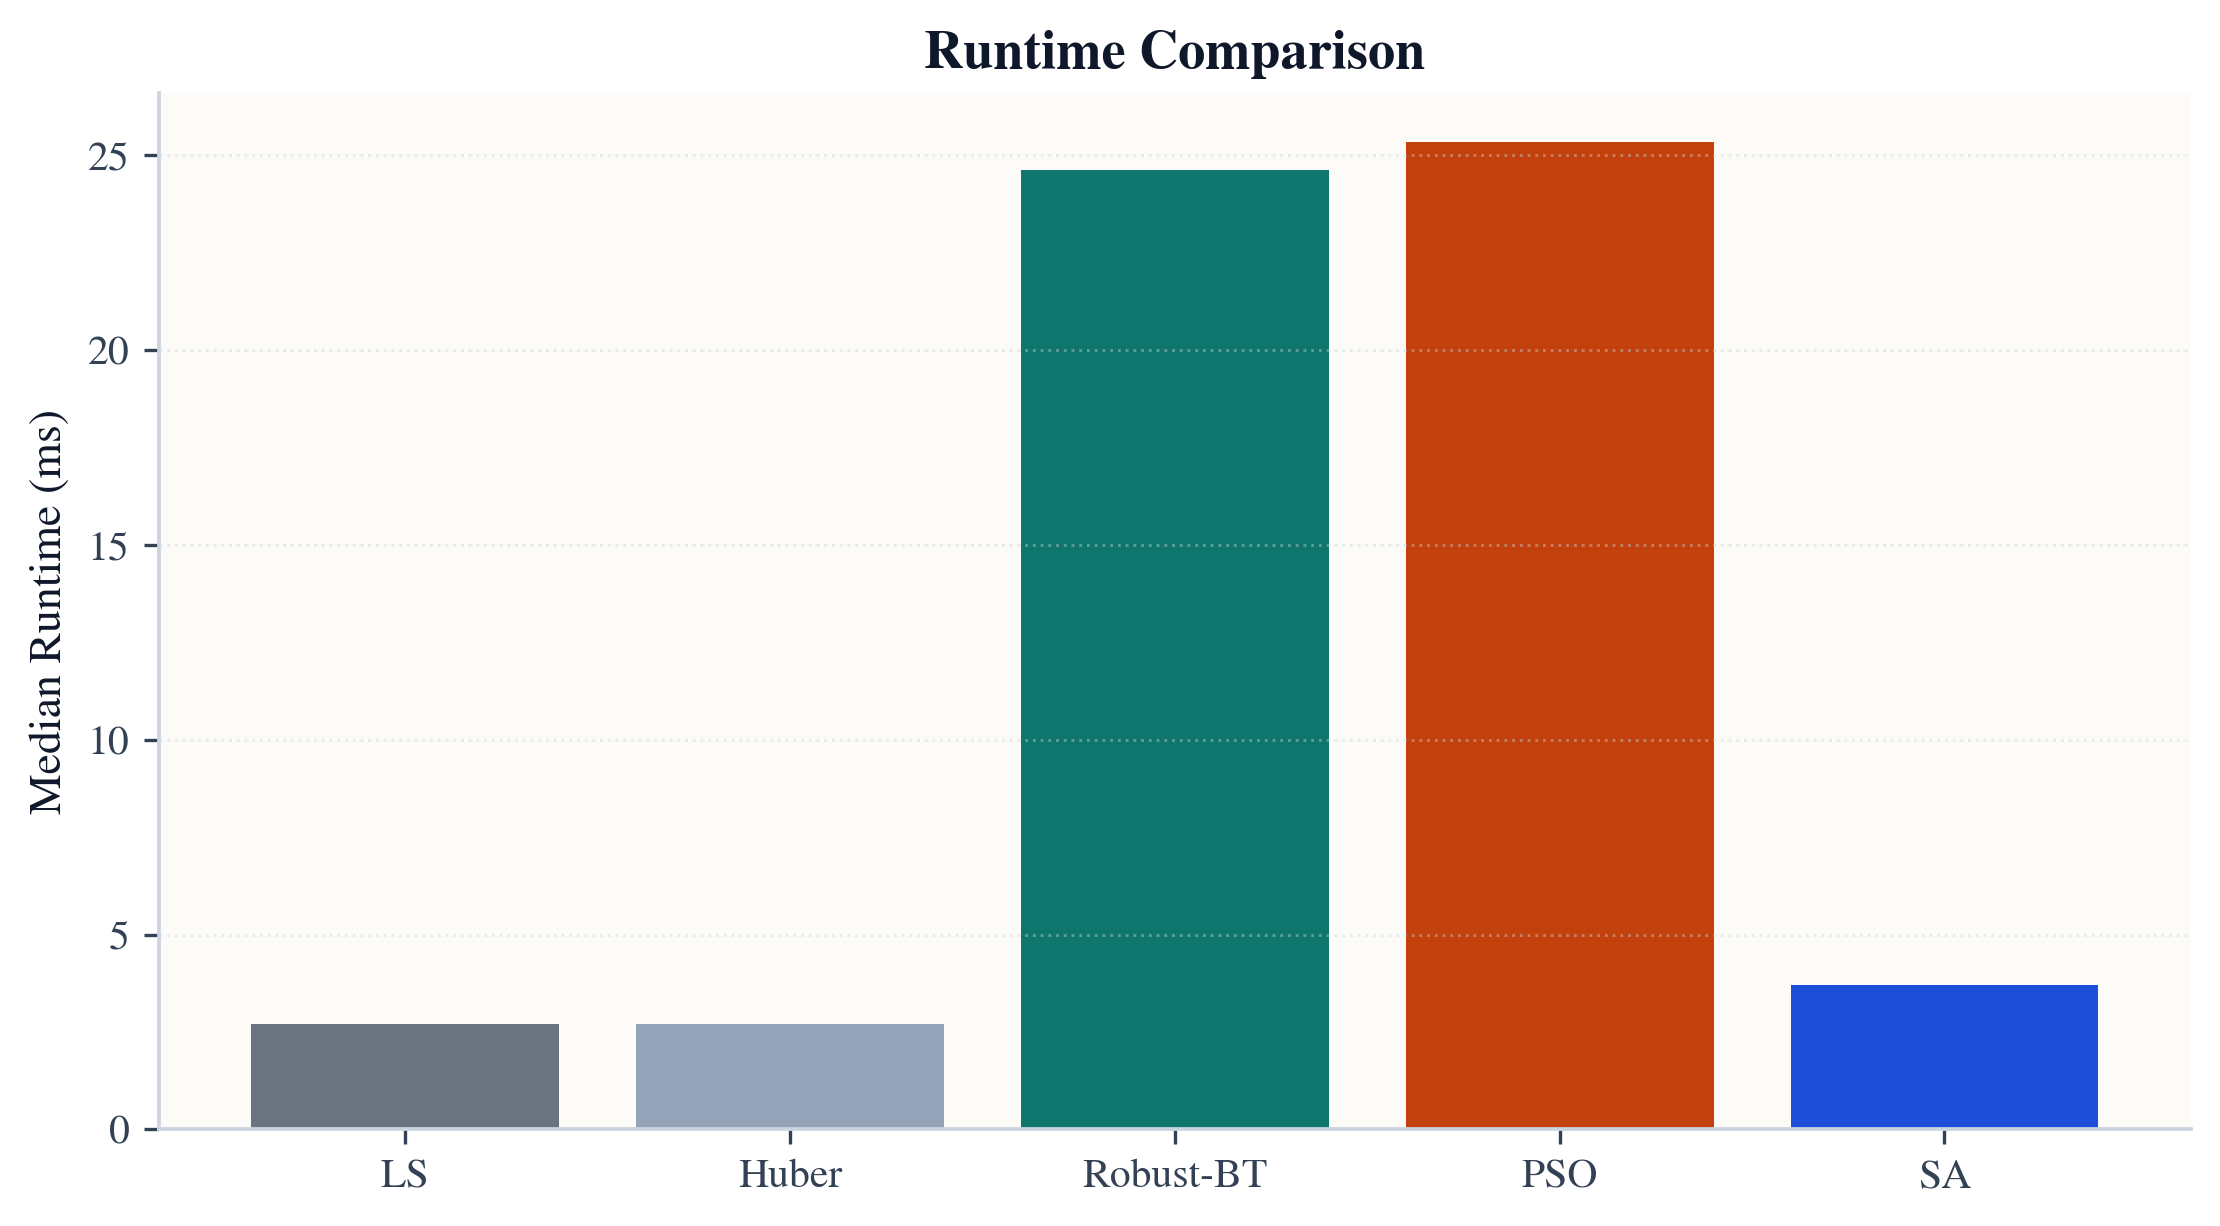
\includegraphics[width=0.75\linewidth]{../figures/figure_runtime_comparison.png}
\caption{Implementation-cost comparison reported for completeness rather than as a primary claim.}
\label{fig:runtime}
\end{figure}

\begin{figure}[t]
\centering
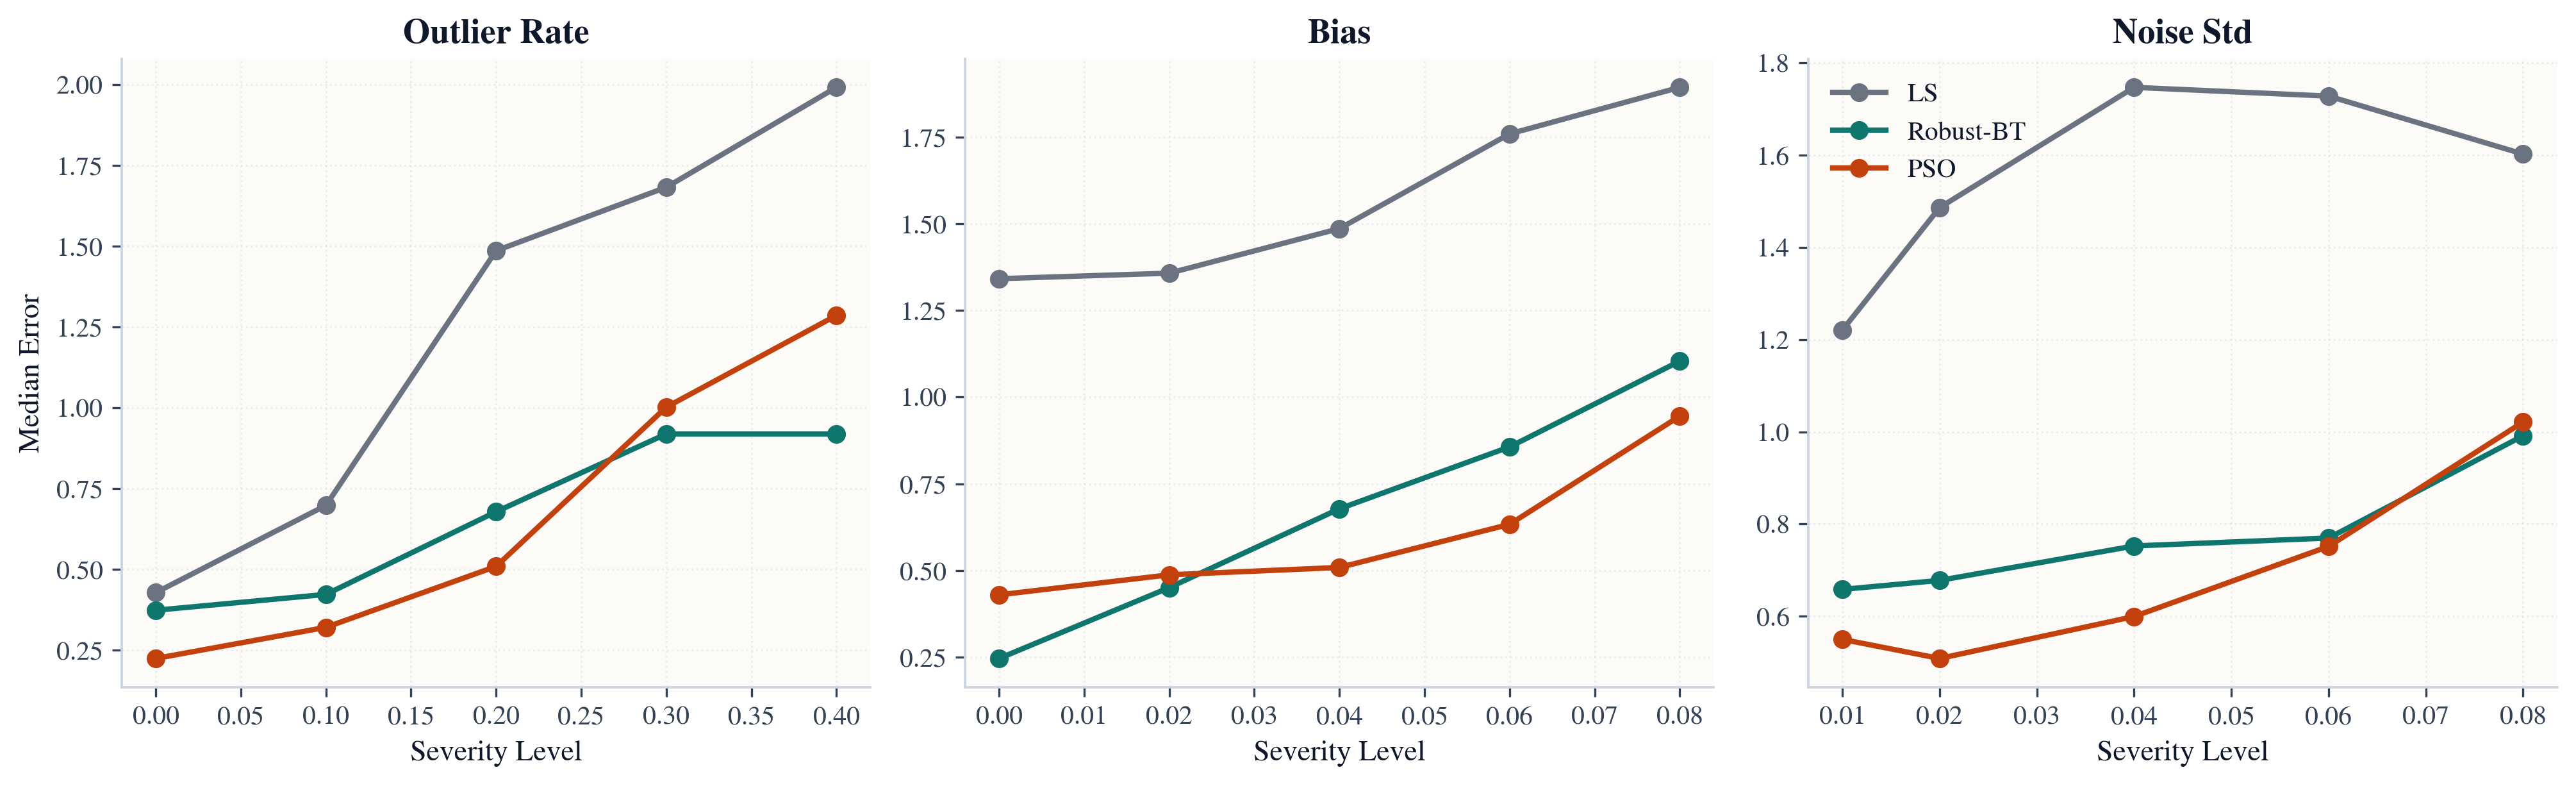
\includegraphics[width=0.98\linewidth]{../figures/figure_sensitivity_sweep.png}
\caption{Sensitivity sweeps over outlier rate, common bias, and nominal noise.}
\label{fig:sensitivity}
\end{figure}

\begin{figure}[t]
\centering
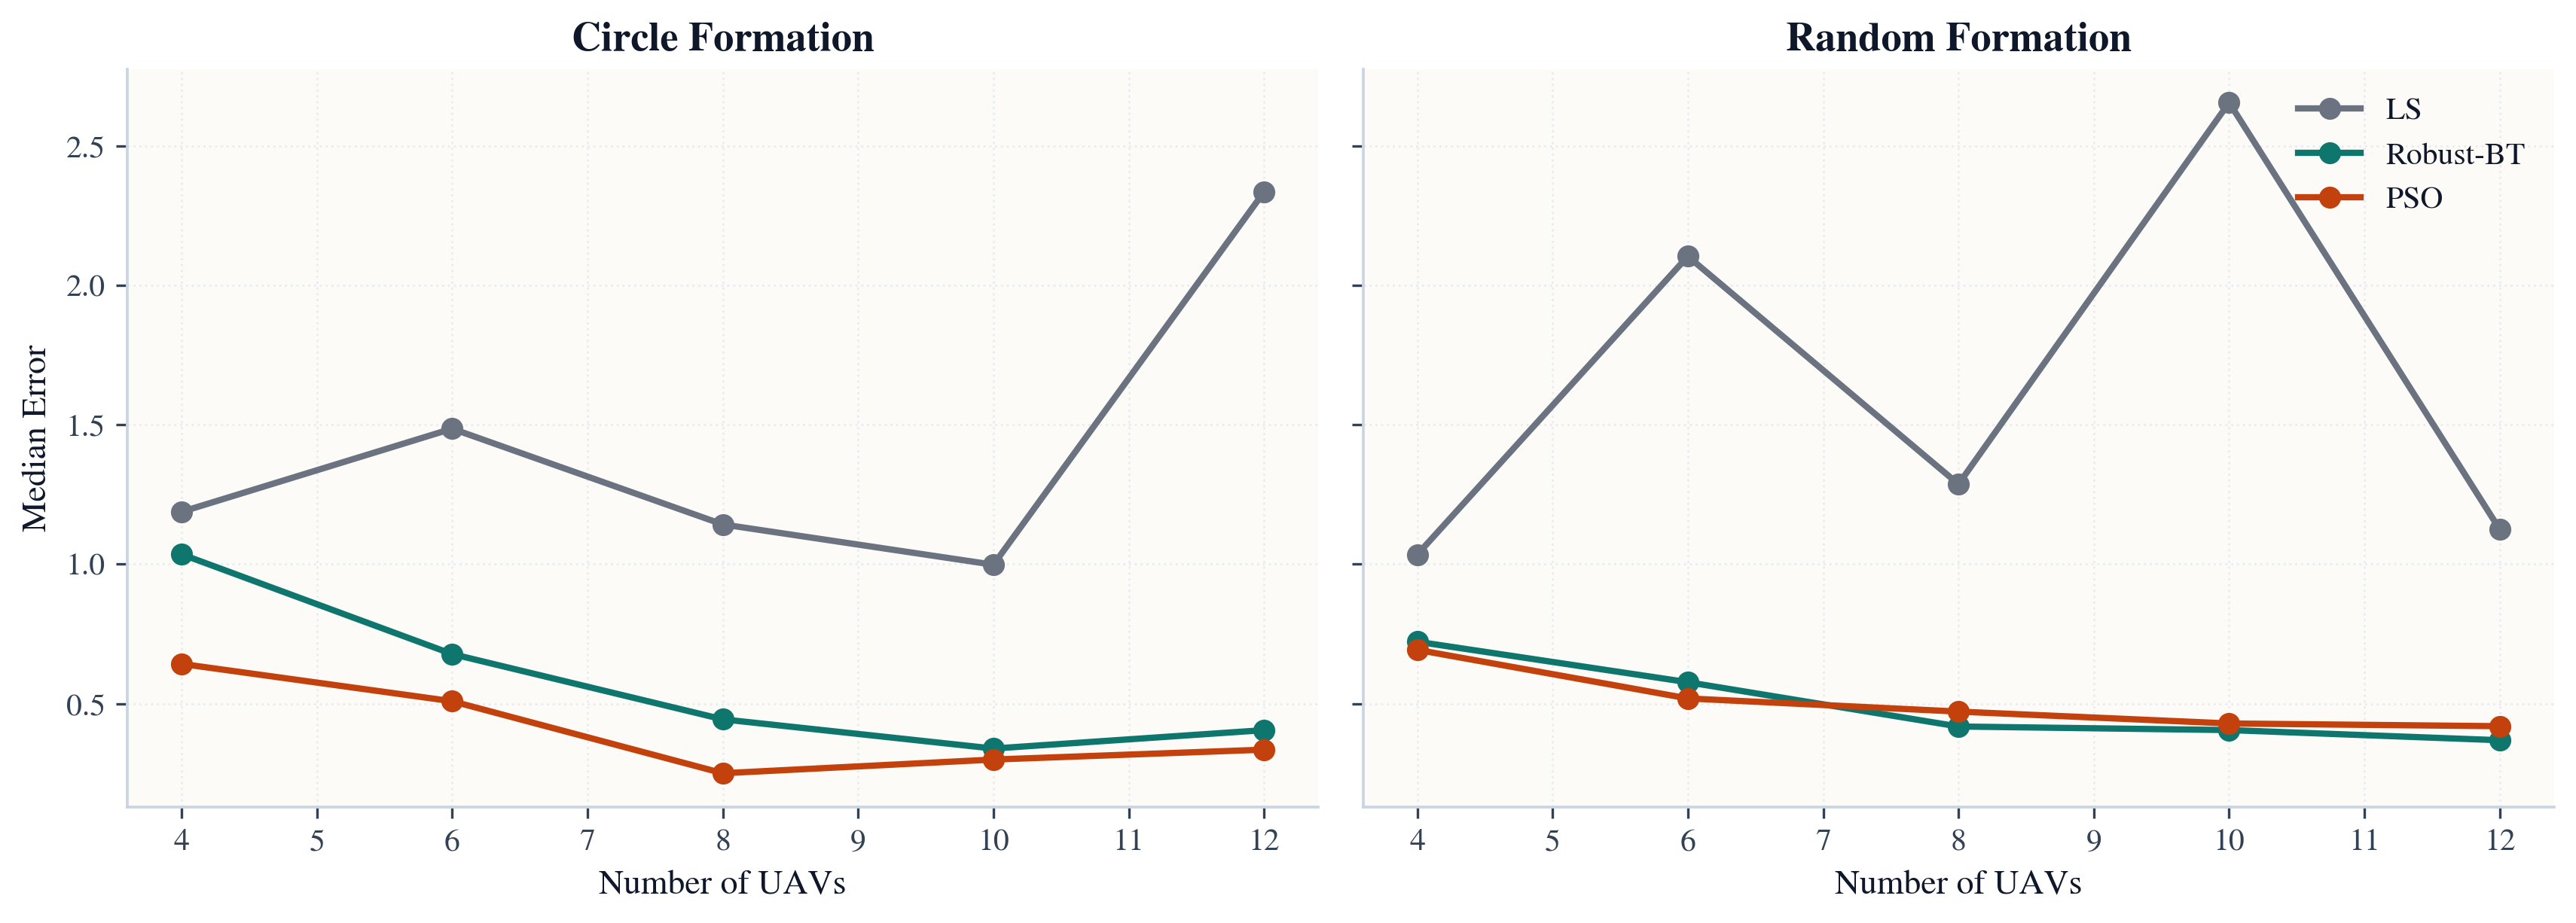
\includegraphics[width=0.98\linewidth]{../figures/figure_scaling.png}
\caption{Sensor-count scaling under circular and random formations.}
\label{fig:scaling}
\end{figure}

\begin{figure}[t]
\centering
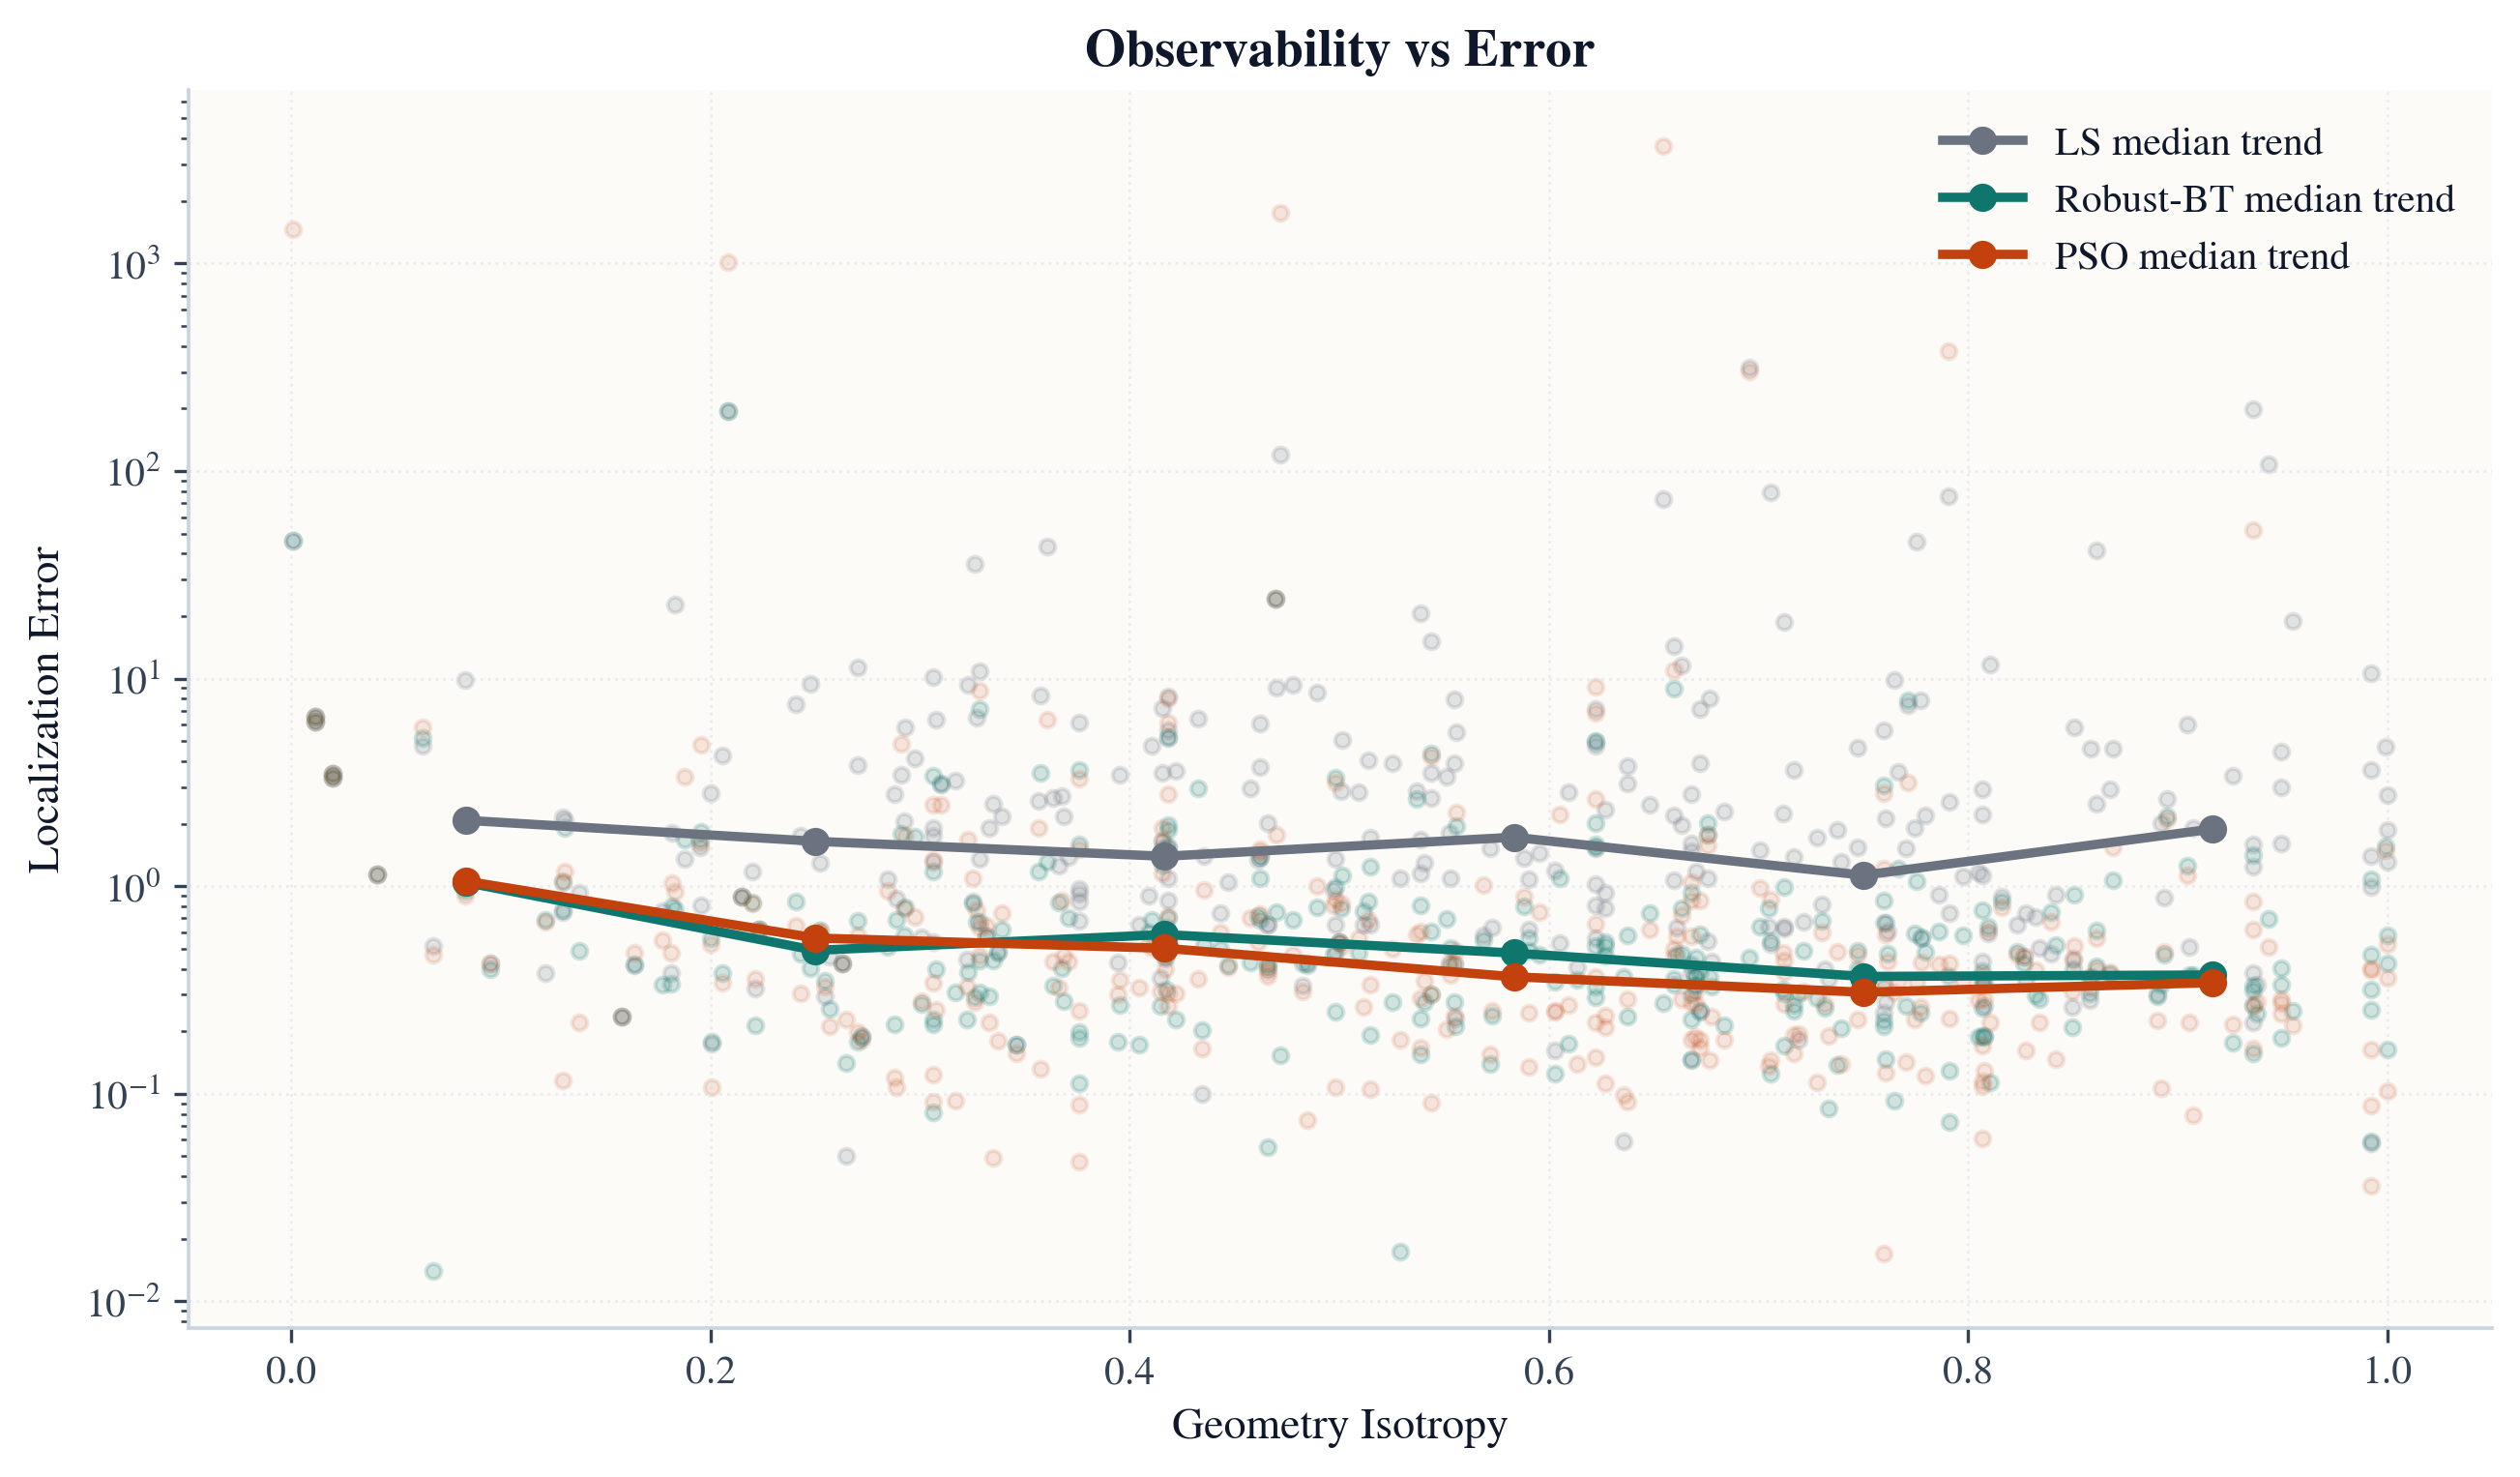
\includegraphics[width=0.84\linewidth]{../figures/figure_observability.png}
\caption{Observability versus error using oracle geometry isotropy for interpretation.}
\label{fig:observability}
\end{figure}

\begin{figure}[t]
\centering
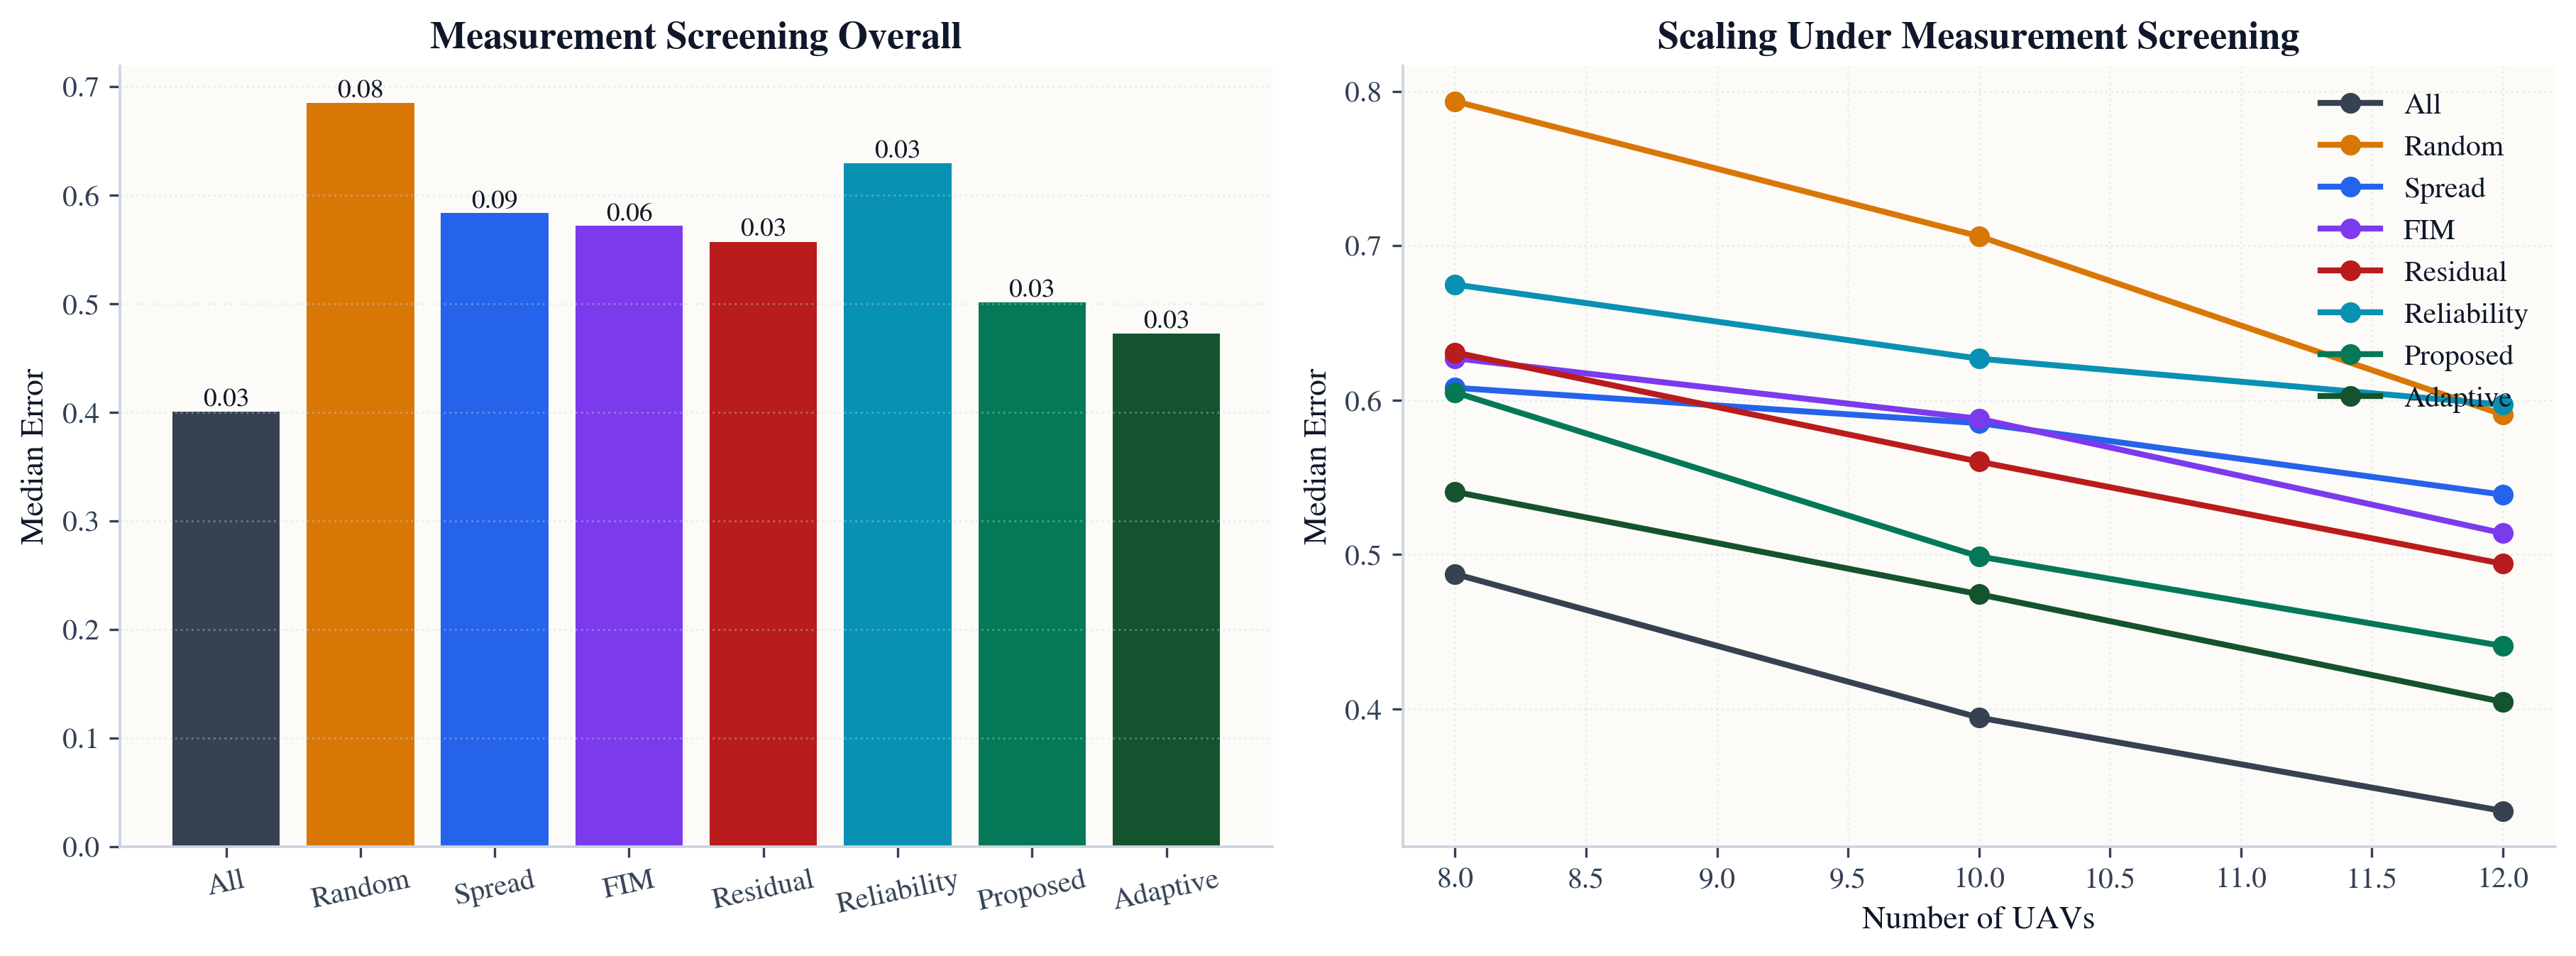
\includegraphics[width=0.98\linewidth]{../figures/figure_active_selection.png}
\caption{Credibility-guided measurement-selection benchmark comparing all-sensor estimation, random subsets, angular-spread greedy selection, FIM/CRLB-greedy selection, and the proposed residual-aware observability policy.}
\label{fig:active}
\end{figure}

% Legacy aggregate table file retained only as a pointer for auditability.
% The current manuscript does not input this file.
% Canonical table sources are the individual submission/tables/table_*.tex files
% and the compiled manuscript at submission/mdpi_manuscript/manuscript_mdpi.pdf.


\section{Discussion}

The paper's most defensible claim is that an interpretable robust passive-localization core is already worthwhile for uncertain measurement conditions. The framework clearly improves over least squares in the degraded regimes that matter most for passive sensing, especially outlier-rich and mixed settings. It also remains competitive with representative heuristic global search without relying entirely on opaque optimization behavior.

The measurement-selection layer further clarifies the practical story. When only a subset of bearings should be trusted or retained, residual-aware selection can outperform random, geometry-only, and FIM-only subset policies. However, the mixed paired comparison against all-sensor estimation also shows that selection should be viewed as a conditional tool, not a universal law. This honesty is important for journal quality because it ties the contribution to a real operational question: not all passive observations are equally useful, and a lighter system may benefit from selecting the most credible ones.

The literature review also shows where stronger future work lies. Recent papers increasingly incorporate observability-aware trajectory design, CRLB-driven path planning, passive node selection, or heavier collaborative inference \cite{peng2024trajectory,chen2025variable,xing2025node,yang2024distributed,li2026formation}. The present study is therefore best positioned as an intermediate but meaningful step: a lightweight uncertainty-aware algorithmic framework, not yet a full system-level active-planning stack.

\section{Conclusion}

This paper presented an uncertainty-aware bearing-only passive localization framework for collaborative UAV sensing under degraded measurements. By combining multi-candidate geometric initialization, trimming-aware residual suppression, iterative reweighted refinement, and a credibility-guided measurement-selection layer, the method improves degraded-regime stability relative to least-squares baselines and outperforms simpler fixed-budget subset policies in the new benchmark. The experiments clarify that the strongest gains occur in outlier-rich and mixed regimes, where the risk of fusing unreliable bearings is highest, and that richer sensing geometry further amplifies those gains.

The work is best understood as a simulation-validated algorithmic framework rather than a complete active-sensing system. Its immediate value is to provide a reusable passive-localization baseline for uncertain observations, together with an honest benchmark that distinguishes robust estimation from measurement selection. Future work should extend the current one-shot selection stage toward sequential planning, richer uncertainty quantification, and hardware or replay-based validation.

\bibliographystyle{elsarticle-num}
\bibliography{references_curated}

\end{document}
